\chapter{Introduction}
\label{introduction}

As the efficiency and accuracy of rapid genome sequencing skyrockets, the potential for personalized therapies has made its way from science fiction to scientific reality. Using genetics to understand, diagnose, and eventually to predict illness is not a new idea; in recent years, however, technological ability and scientific understanding have advanced to such a point that researchers may predict risk for several diseases with reasonable confidence. Increasingly, variants in the human genome are being identified as being robustly linked to risk for complex illnesses such as heart disease [\small{cite 9p21}], obesity [\small{cite fto}], and schizophrenia [\small{cite something}]. However, much work remains to be done in order to create tools which may accurately predict individual disease risk from known and unknown genetic risk factors. In this thesis, we propose a novel extension to a well known methodology in order to better characterize disease risk from comorbid conditions using only summary statistics. 

In brief, we present preliminary evidence for the use of \ac{PRS}s in predicting \ac{CAD}. We use recently published summary statistics from a \ac{GWAS} conducted by the \ac{CARDIOGRAMC4D} consortium alongside evidence gathered by the \ac{GLC} and the \ac{GIANT} consortium for lipids and \ac{BMI} \textit{per say}. We use this data alongside previously identified variants to construct first a simplistic \ac{PRS} using only genome wide statistically signficant ($P_{Bonferonni} < 0.05$ or $q_{FDR}$ < 0.05) variants, then expand our search to variants which may not be as robustly linked to phenotype. [Cite storey, BH, and dudbridge]. We use an empirical maximation approach and several strategies of mathematical optimization in order to construct an \ac{oPRS}, then devise a novel technique for integrating information from co-morbid \ac{oPRS} diseases in order to better predict \ac{CAD} in four cohorts comprising approximately $n=12,000$ individuals

\section{Genetics of Coronary Artery Disease}

\ac{CAD} occurs when the major blood vessels supplying the heart become diseased or damaged, often leading to severe complications such as \ac{MI} and death. [cite review articles] \ac{CAD} is known to be a complex genetic disease with heritability estimated by twin studies between 40 and 60\%. [mcPherson 2016, twin studies paper] Several important variants have been indentified which have been shown to robustly increase risk to \ac{CAD} by altering lipid transporting pathways [cite LDLR], structural collegan bodies [TRIB 1??], and others factors. 


\begin{figure}[h]
\caption{Progression of the formation of plaque causing \ac{CAD}. Adapted from Gretch 2003.}
\centering
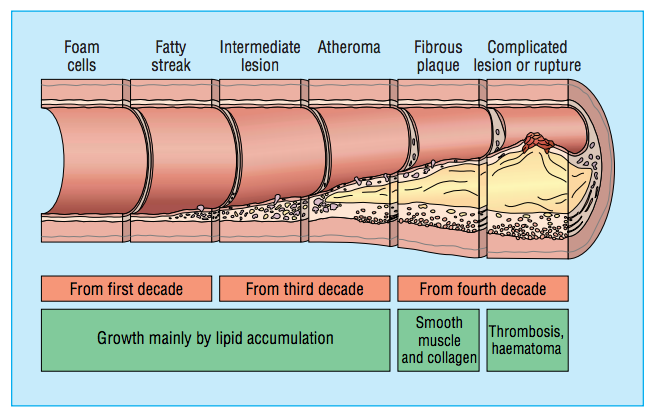
\includegraphics[width=0.8\textwidth]{Figures/cad.png}
\end{figure}



With heart disease and stroke the leading cause of perscription drug use in Canada as well as one of the leading causes of death and hospitalization [cite herat and stroke], the need to better understand, diagnose, and prevent this deadly disease is apparent.  In order to better understand the need for improved statistical methodologies, it is important to understand the large body of previous attempts to characterize the genetic determinants of \ac{CAD}

Despite some promising beginings, initial attempts to understand and explain \ac{CAD} through genetics were largely unsuccessful.[CITE] The first variant to be succesfully and robustly linked to risk for \ac{CAD} was the 9p21.3 locus. Discovered by a team of researchers at the Univeristy of Ottawa Heart institute, the allele consists of a 58 \ac{kb} region on chromosome 9 which was shown to be associated with \ac{CAD} in a population of 23,000 caucasion individuals. (\cite{McPherson2016})

\begin{figure}[h]
\caption{Fine mapping of the genomic interval on chromosome 9 associated with Coronary Heart Disease. Adapted from Mcpherson et al 2006}
\centering
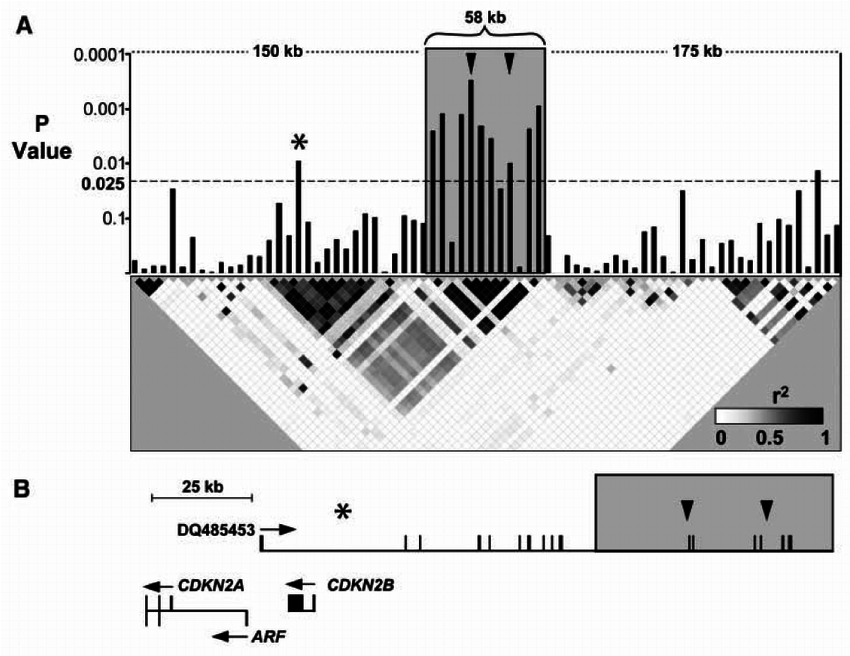
\includegraphics[width=0.8\textwidth]{Figures/9p21.png}
\end{figure}

This initial success began the era of the \ac{GWAS}, explained in more detail in section \ref{gwas}, which paved the way


\section{Genome Wide Association Studies} \label{gwas}
\section{Polygenic Prediction of Complex Disease}
\section{Polygenic Sliding Window Optimization}
\section{Summary}